% !TeX root = ../../tesis.tex

% -----------------------------------------------------------------------
\subsection{Robustez Geométrica --- Vulnerabilidad \texorpdfstring{($\Delta E$)}{(Delta E)}}
\label{subsec:robustez-geometrica}
% -----------------------------------------------------------------------

\textbf{Fuente principal:} \citet{lotero2014vulnerabilidad}

\subsubsection{Definición y Fundamentación}

La Robustez Geométrica es el indicador de mayor dependencia jerárquica del
modelo: para calcularlo, se requiere conocer previamente qué nodo destruir
---dado por el Indicador de Centralidad de Intermediación (
\autoref{subsec:centralidad-intermediacion})--- y medir el impacto de esa
destrucción sobre el desempeño global ---dado por el Indicador de Tiempo de
Viaje Promedio (\autoref{subsec:tiempo-viaje})---.

\citet{lotero2014vulnerabilidad} definen la vulnerabilidad operativamente como
la disminución de la eficiencia de la red después de un ataque o falla. La
metodología estándar para medir la robustez consiste en cuantificar el impacto
de la remoción de un componente de la red, ya sea de forma aleatoria
---simulando una falla fortuita como el cierre de una estación por inundación o
mantenimiento--- o de forma dirigida hacia los elementos más importantes,
simulando un ataque a un nodo crítico. Los autores señalan que las redes con
distribución libre de escala son robustas ante fallas aleatorias, pero altamente
vulnerables ante ataques dirigidos a sus nodos más conectados, resultado que es
la base teórica del experimento de fase final del presente trabajo.

\subsubsection{Fórmula}

\begin{equation}
    \Delta E = \frac{E_0 - E_f}{E_0}
    \label{eq:robustez}
\end{equation}

Donde:
\begin{itemize}
\item $\Delta E$ = Caída relativa de eficiencia de la red tras la remoción de un
    nodo o conjunto de nodos (adimensional, rango $[0, 1]$).
\item $E_0$ = Eficiencia global de la red en el estado completo, expresada como
    el inverso del Tiempo de Viaje Promedio:
    $E_0 = 1 / T_{\text{completa}}$.
\item $E_f$ = Eficiencia global de la red en el estado fallido (tras la remoción
    del nodo o nodos críticos):
    $E_f = 1 / T_{\text{fallida}}$.
\end{itemize}

Un valor $\Delta E \approx 0$ indica que la red es robusta: la pérdida del nodo
no afecta significativamente el desempeño global (existen rutas alternativas
eficientes). Un valor $\Delta E \to 1$ indica que la red es frágil: la pérdida
de ese nodo produce una degradación severa del servicio.


\begin{figure}[H]
    \centering
    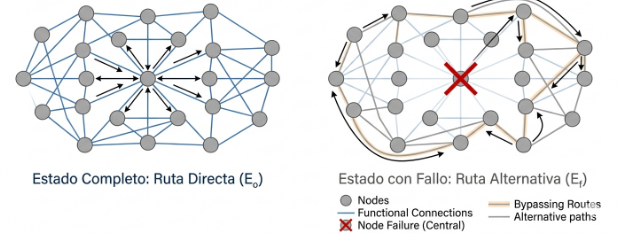
\includegraphics[width=0.80\textwidth]{Figures/Cap3/RobustezGeometrica.png}
    \caption[Diagrama del indicador de Robustez Geométrica $\Delta E$]{Estado
    completo con ruta directa ($E_0$) versus estado con fallo y rutas
    alternativas de desvío ($E_f$).}
    \label{fig:indicador-deltaE}
    \fuentefigura{Elaboración propia con base en \citet{lotero2014vulnerabilidad}.}
\end{figure}


\subsubsection{Ejemplo Práctico: \cdmx{} y Zona Metropolitana}

\textbf{Experimento:} Remoción del nodo ``Pantitlán'' (nodo de mayor $B(v)$ en
la red actual).

\begin{table}[H]
    \centering
    \caption{Impacto del indicador $\Delta E$ ante la remoción de Pantitlán.}
    \label{tab:robustez}
    \begin{tabularx}{\textwidth}{X r r r}
        \toprule
        \textbf{Condición} & \textbf{$T$ promedio} &
        \textbf{$E = 1/T$} & \textbf{$\Delta E$} \\
        \midrule
        Red actual completa ($E_0$)          & 85 min & 0.01176 & --- \\
        Red actual sin Pantitlán ($E_f$)     & 133 min & 0.00752 & $\mathbf{36\%}$ \\
        Red con Anillo completo ($E_0'$)     & 65 min & 0.01538 & --- \\
        Red con Anillo sin Pantitlán ($E_f'$) & 78 min & 0.01282 & $\mathbf{17\%}$ \\
        \bottomrule
    \end{tabularx}
\end{table}

La diferencia entre $\Delta E = 36\%$ (red radial sin anillo) y
$\Delta E = 17\% $ (red con anillo periférico) demuestra algorítmicamente que la
propuesta reduce la vulnerabilidad del sistema ante la pérdida del nodo más
crítico en casi un 53\%, dotando a la red metropolitana de redundancia
estructural.

La implementación computacional de referencia para este indicador se encuentra
en el \autoref{anx:indicadores-implementacion} (§\ref{anx:impl-robustez}).
Conforme a la nota aclaratoria de §\ref{sec:indicadores-formulas}, la validación
empírica de $\Delta E$ queda propuesta como línea de investigación futura.

El indicador $\Delta E$ articula los Objetivos Específicos 3 y 5 (§
\ref{subsec:obj-especificos}): la comparación de $\Delta E_{\text{actual}}$ con
$\Delta E_{\text{anillo}}$ ante la remoción de los nodos más críticos del
sistema demuestra si el corredor anillar propuesto reduce efectivamente la
fragilidad de la red, dotándola de rutas alternativas capaces de absorber la
demanda desplazada. Es, en este sentido, el indicador que cierra el argumento de
la investigación al ligar la hipótesis urbanística con la demostración
algorítmica.
